\documentclass[1p]{elsarticle_modified}
%\bibliographystyle{elsarticle-num}

%\usepackage[colorlinks]{hyperref}
%\usepackage{abbrmath_seonhwa} %\Abb, \Ascr, \Acal ,\Abf, \Afrak
\usepackage{amsfonts}
\usepackage{amssymb}
\usepackage{amsmath}
\usepackage{amsthm}
\usepackage{scalefnt}
\usepackage{amsbsy}
\usepackage{kotex}
\usepackage{caption}
\usepackage{subfig}
\usepackage{color}
\usepackage{graphicx}
\usepackage{xcolor} %% white, black, red, green, blue, cyan, magenta, yellow
\usepackage{float}
\usepackage{setspace}
\usepackage{hyperref}

\usepackage{tikz}
\usetikzlibrary{arrows}

\usepackage{multirow}
\usepackage{array} % fixed length table
\usepackage{hhline}

%%%%%%%%%%%%%%%%%%%%%
\makeatletter
\renewcommand*\env@matrix[1][\arraystretch]{%
	\edef\arraystretch{#1}%
	\hskip -\arraycolsep
	\let\@ifnextchar\new@ifnextchar
	\array{*\c@MaxMatrixCols c}}
\makeatother %https://tex.stackexchange.com/questions/14071/how-can-i-increase-the-line-spacing-in-a-matrix
%%%%%%%%%%%%%%%

\usepackage[normalem]{ulem}

\newcommand{\msout}[1]{\ifmmode\text{\sout{\ensuremath{#1}}}\else\sout{#1}\fi}
%SOURCE: \msout is \stkout macro in https://tex.stackexchange.com/questions/20609/strikeout-in-math-mode

\newcommand{\cancel}[1]{
	\ifmmode
	{\color{red}\msout{#1}}
	\else
	{\color{red}\sout{#1}}
	\fi
}

\newcommand{\add}[1]{
	{\color{blue}\uwave{#1}}
}

\newcommand{\replace}[2]{
	\ifmmode
	{\color{red}\msout{#1}}{\color{blue}\uwave{#2}}
	\else
	{\color{red}\sout{#1}}{\color{blue}\uwave{#2}}
	\fi
}

\newcommand{\Sol}{\mathcal{S}} %segment
\newcommand{\D}{D} %diagram
\newcommand{\A}{\mathcal{A}} %arc


%%%%%%%%%%%%%%%%%%%%%%%%%%%%%5 test

\def\sl{\operatorname{\textup{SL}}(2,\Cbb)}
\def\psl{\operatorname{\textup{PSL}}(2,\Cbb)}
\def\quan{\mkern 1mu \triangleright \mkern 1mu}

\theoremstyle{definition}
\newtheorem{thm}{Theorem}[section]
\newtheorem{prop}[thm]{Proposition}
\newtheorem{lem}[thm]{Lemma}
\newtheorem{ques}[thm]{Question}
\newtheorem{cor}[thm]{Corollary}
\newtheorem{defn}[thm]{Definition}
\newtheorem{exam}[thm]{Example}
\newtheorem{rmk}[thm]{Remark}
\newtheorem{alg}[thm]{Algorithm}

\newcommand{\I}{\sqrt{-1}}
\begin{document}

%\begin{frontmatter}
%
%\title{Boundary parabolic representations of knots up to 8 crossings}
%
%%% Group authors per affiliation:
%\author{Yunhi Cho} 
%\address{Department of Mathematics, University of Seoul, Seoul, Korea}
%\ead{yhcho@uos.ac.kr}
%
%
%\author{Seonhwa Kim} %\fnref{s_kim}}
%\address{Center for Geometry and Physics, Institute for Basic Science, Pohang, 37673, Korea}
%\ead{ryeona17@ibs.re.kr}
%
%\author{Hyuk Kim}
%\address{Department of Mathematical Sciences, Seoul National University, Seoul 08826, Korea}
%\ead{hyukkim@snu.ac.kr}
%
%\author{Seokbeom Yoon}
%\address{Department of Mathematical Sciences, Seoul National University, Seoul, 08826,  Korea}
%\ead{sbyoon15@snu.ac.kr}
%
%\begin{abstract}
%We find all boundary parabolic representation of knots up to 8 crossings.
%
%\end{abstract}
%\begin{keyword}
%    \MSC[2010] 57M25 
%\end{keyword}
%
%\end{frontmatter}

%\linenumbers
%\tableofcontents
%
\newcommand\colored[1]{\textcolor{white}{\rule[-0.35ex]{0.8em}{1.4ex}}\kern-0.8em\color{red} #1}%
%\newcommand\colored[1]{\textcolor{white}{ #1}\kern-2.17ex	\textcolor{white}{ #1}\kern-1.81ex	\textcolor{white}{ #1}\kern-2.15ex\color{red}#1	}

{\Large $\underline{12a_{0080}~(K12a_{0080})}$}

\setlength{\tabcolsep}{10pt}
\renewcommand{\arraystretch}{1.6}
\vspace{1cm}\begin{tabular}{m{100pt}>{\centering\arraybackslash}m{274pt}}
\multirow{5}{120pt}{
	\centering
	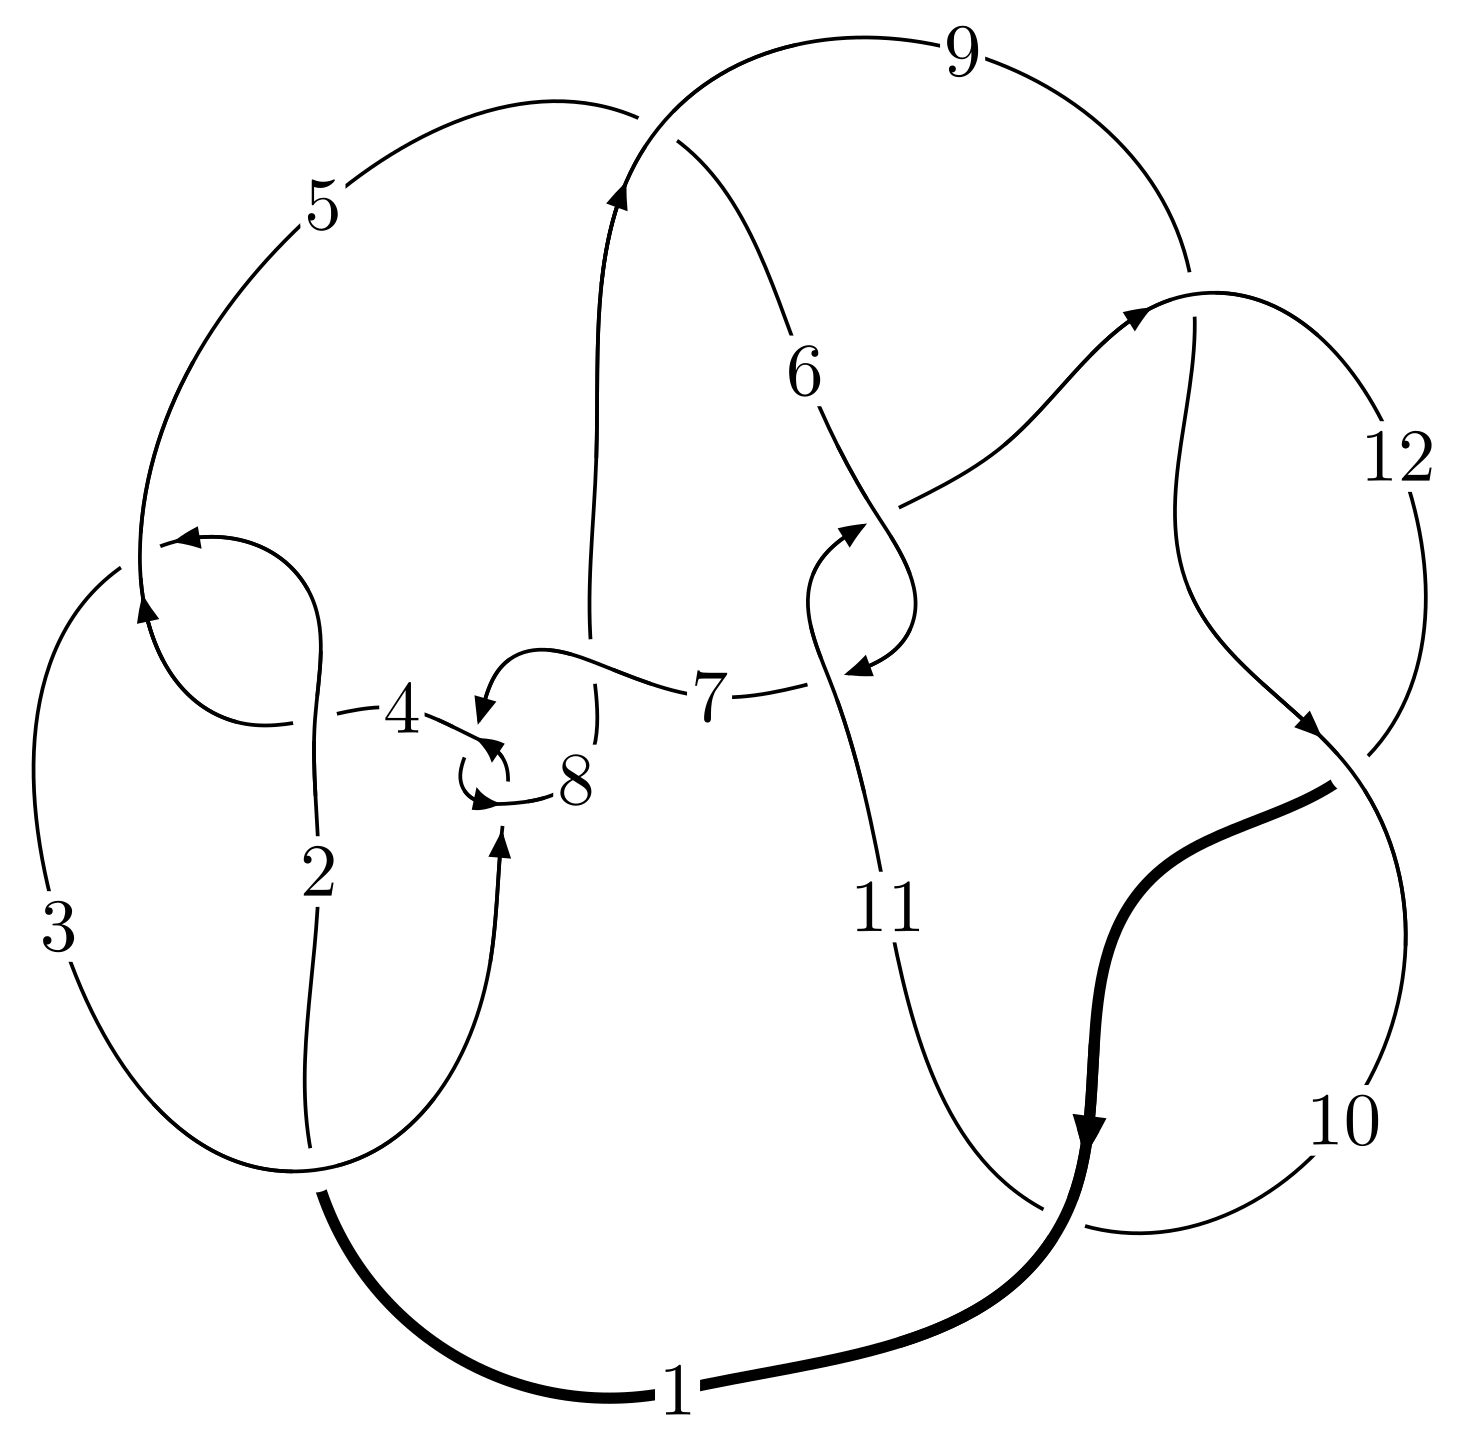
\includegraphics[width=112pt]{../../../GIT/diagram.site/Diagrams/png/881_12a_0080.png}\\
\ \ \ A knot diagram\footnotemark}&
\allowdisplaybreaks
\textbf{Linearized knot diagam} \\
\cline{2-2}
 &
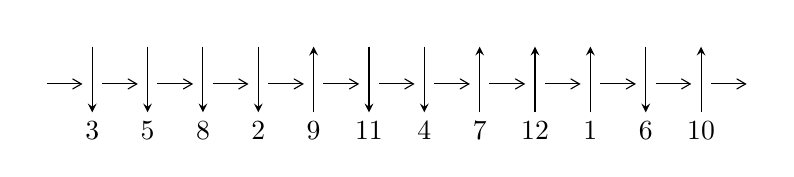
\begin{tikzpicture}[x=20pt, y=17pt]
	% nodes
	\node (C0) at (0, 0) {};
	\node (C1) at (1, 0) {};
	\node (C1U) at (1, +1) {};
	\node (C1D) at (1, -1) {3};

	\node (C2) at (2, 0) {};
	\node (C2U) at (2, +1) {};
	\node (C2D) at (2, -1) {5};

	\node (C3) at (3, 0) {};
	\node (C3U) at (3, +1) {};
	\node (C3D) at (3, -1) {8};

	\node (C4) at (4, 0) {};
	\node (C4U) at (4, +1) {};
	\node (C4D) at (4, -1) {2};

	\node (C5) at (5, 0) {};
	\node (C5U) at (5, +1) {};
	\node (C5D) at (5, -1) {9};

	\node (C6) at (6, 0) {};
	\node (C6U) at (6, +1) {};
	\node (C6D) at (6, -1) {11};

	\node (C7) at (7, 0) {};
	\node (C7U) at (7, +1) {};
	\node (C7D) at (7, -1) {4};

	\node (C8) at (8, 0) {};
	\node (C8U) at (8, +1) {};
	\node (C8D) at (8, -1) {7};

	\node (C9) at (9, 0) {};
	\node (C9U) at (9, +1) {};
	\node (C9D) at (9, -1) {12};

	\node (C10) at (10, 0) {};
	\node (C10U) at (10, +1) {};
	\node (C10D) at (10, -1) {1};

	\node (C11) at (11, 0) {};
	\node (C11U) at (11, +1) {};
	\node (C11D) at (11, -1) {6};

	\node (C12) at (12, 0) {};
	\node (C12U) at (12, +1) {};
	\node (C12D) at (12, -1) {10};
	\node (C13) at (13, 0) {};

	% arrows
	\draw[->,>={angle 60}]
	(C0) edge (C1) (C1) edge (C2) (C2) edge (C3) (C3) edge (C4) (C4) edge (C5) (C5) edge (C6) (C6) edge (C7) (C7) edge (C8) (C8) edge (C9) (C9) edge (C10) (C10) edge (C11) (C11) edge (C12) (C12) edge (C13) ;	\draw[->,>=stealth]
	(C1U) edge (C1D) (C2U) edge (C2D) (C3U) edge (C3D) (C4U) edge (C4D) (C5D) edge (C5U) (C6U) edge (C6D) (C7U) edge (C7D) (C8D) edge (C8U) (C9D) edge (C9U) (C10D) edge (C10U) (C11U) edge (C11D) (C12D) edge (C12U) ;
	\end{tikzpicture} \\
\hhline{~~} \\& 
\textbf{Solving Sequence} \\ \cline{2-2} 
 &
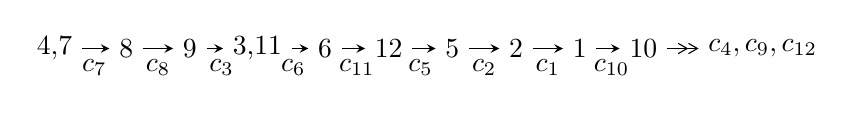
\begin{tikzpicture}[x=23pt, y=7pt]
	% node
	\node (A0) at (-1/8, 0) {4,7};
	\node (A1) at (1, 0) {8};
	\node (A2) at (2, 0) {9};
	\node (A3) at (49/16, 0) {3,11};
	\node (A4) at (33/8, 0) {6};
	\node (A5) at (41/8, 0) {12};
	\node (A6) at (49/8, 0) {5};
	\node (A7) at (57/8, 0) {2};
	\node (A8) at (65/8, 0) {1};
	\node (A9) at (73/8, 0) {10};
	\node (C1) at (1/2, -1) {$c_{7}$};
	\node (C2) at (3/2, -1) {$c_{8}$};
	\node (C3) at (5/2, -1) {$c_{3}$};
	\node (C4) at (29/8, -1) {$c_{6}$};
	\node (C5) at (37/8, -1) {$c_{11}$};
	\node (C6) at (45/8, -1) {$c_{5}$};
	\node (C7) at (53/8, -1) {$c_{2}$};
	\node (C8) at (61/8, -1) {$c_{1}$};
	\node (C9) at (69/8, -1) {$c_{10}$};
	\node (A10) at (11, 0) {$c_{4},c_{9},c_{12}$};

	% edge
	\draw[->,>=stealth]	
	(A0) edge (A1) (A1) edge (A2) (A2) edge (A3) (A3) edge (A4) (A4) edge (A5) (A5) edge (A6) (A6) edge (A7) (A7) edge (A8) (A8) edge (A9) ;
	\draw[->>,>={angle 60}]	
	(A9) edge (A10);
\end{tikzpicture} \\ 

\end{tabular} \\

\footnotetext{
The image of knot diagram is generated by the software ``\textbf{Draw programme}" developed by Andrew Bartholomew(\url{http://www.layer8.co.uk/maths/draw/index.htm\#Running-draw}), where we modified some parts for our purpose(\url{https://github.com/CATsTAILs/LinksPainter}).
}\phantom \\ \newline 
\centering \textbf{Ideals for irreducible components\footnotemark of $X_{\text{par}}$} 
 
\begin{align*}
I^u_{1}&=\langle 
2.47932\times10^{172} u^{99}+4.76140\times10^{172} u^{98}+\cdots+7.64219\times10^{171} b-7.86042\times10^{173},\\
\phantom{I^u_{1}}&\phantom{= \langle  }1.61477\times10^{173} u^{99}+2.13974\times10^{173} u^{98}+\cdots+1.52844\times10^{172} a-2.14797\times10^{174},\\
\phantom{I^u_{1}}&\phantom{= \langle  }u^{100}+2 u^{99}+\cdots-64 u-32\rangle \\
I^u_{2}&=\langle 
b,\;- u^8+2 u^7-3 u^6+3 u^5-4 u^4+4 u^3-3 u^2+a+2 u-1,\;u^9- u^8+2 u^7- u^6+3 u^5- u^4+2 u^3+u+1\rangle \\
\\
I^v_{1}&=\langle 
a,\;2 v^4- v^3-3 v^2+b+6 v-2,\;v^5- v^4- v^3+4 v^2-3 v+1\rangle \\
\end{align*}
\raggedright * 3 irreducible components of $\dim_{\mathbb{C}}=0$, with total 114 representations.\\
\footnotetext{All coefficients of polynomials are rational numbers. But the coefficients are sometimes approximated in decimal forms when there is not enough margin.}
\newpage
\renewcommand{\arraystretch}{1}
\centering \section*{I. $I^u_{1}= \langle 2.48\times10^{172} u^{99}+4.76\times10^{172} u^{98}+\cdots+7.64\times10^{171} b-7.86\times10^{173},\;1.61\times10^{173} u^{99}+2.14\times10^{173} u^{98}+\cdots+1.53\times10^{172} a-2.15\times10^{174},\;u^{100}+2 u^{99}+\cdots-64 u-32 \rangle$}
\flushleft \textbf{(i) Arc colorings}\\
\begin{tabular}{m{7pt} m{180pt} m{7pt} m{180pt} }
\flushright $a_{4}=$&$\begin{pmatrix}0\\u\end{pmatrix}$ \\
\flushright $a_{7}=$&$\begin{pmatrix}1\\0\end{pmatrix}$ \\
\flushright $a_{8}=$&$\begin{pmatrix}1\\u^2\end{pmatrix}$ \\
\flushright $a_{9}=$&$\begin{pmatrix}u^2+1\\u^2\end{pmatrix}$ \\
\flushright $a_{3}=$&$\begin{pmatrix}u\\u^3+u\end{pmatrix}$ \\
\flushright $a_{11}=$&$\begin{pmatrix}-10.5648 u^{99}-13.9996 u^{98}+\cdots+485.144 u+140.533\\-3.24425 u^{99}-6.23041 u^{98}+\cdots+227.295 u+102.856\end{pmatrix}$ \\
\flushright $a_{6}=$&$\begin{pmatrix}-1.62635 u^{99}-12.7491 u^{98}+\cdots+379.363 u+373.535\\2.75906 u^{99}-1.00208 u^{98}+\cdots+17.4499 u+112.614\end{pmatrix}$ \\
\flushright $a_{12}=$&$\begin{pmatrix}1.99211 u^{99}-0.362984 u^{98}+\cdots+11.6286 u+92.4955\\4.80922 u^{99}+8.87550 u^{98}+\cdots-249.660 u-114.564\end{pmatrix}$ \\
\flushright $a_{5}=$&$\begin{pmatrix}-2.00742 u^{99}-6.91461 u^{98}+\cdots+214.739 u+175.776\\-2.72976 u^{99}-5.69852 u^{98}+\cdots+201.086 u+122.708\end{pmatrix}$ \\
\flushright $a_{2}=$&$\begin{pmatrix}-6.01213 u^{99}-5.95088 u^{98}+\cdots+236.170 u+39.7247\\-9.17264 u^{99}-20.1928 u^{98}+\cdots+647.217 u+409.849\end{pmatrix}$ \\
\flushright $a_{1}=$&$\begin{pmatrix}-0.722339 u^{99}+1.21609 u^{98}+\cdots-13.6525 u-53.0678\\-5.10774 u^{99}-10.5309 u^{98}+\cdots+348.261 u+207.853\end{pmatrix}$ \\
\flushright $a_{10}=$&$\begin{pmatrix}-2.75020 u^{99}-1.20374 u^{98}+\cdots+54.2989 u-54.5712\\-1.57899 u^{99}-0.971002 u^{98}+\cdots+14.8200 u-34.6674\end{pmatrix}$\\&\end{tabular}
\flushleft \textbf{(ii) Obstruction class $= -1$}\\~\\
\flushleft \textbf{(iii) Cusp Shapes $= 0.0436322 u^{99}+11.7279 u^{98}+\cdots-467.357 u-260.647$}\\~\\
\newpage\renewcommand{\arraystretch}{1}
\flushleft \textbf{(iv) u-Polynomials at the component}\newline \\
\begin{tabular}{m{50pt}|m{274pt}}
Crossings & \hspace{64pt}u-Polynomials at each crossing \\
\hline $$\begin{aligned}c_{1}\end{aligned}$$&$\begin{aligned}
&u^{100}+53 u^{99}+\cdots+7 u+1
\end{aligned}$\\
\hline $$\begin{aligned}c_{2},c_{4}\end{aligned}$$&$\begin{aligned}
&u^{100}-7 u^{99}+\cdots-7 u+1
\end{aligned}$\\
\hline $$\begin{aligned}c_{3},c_{7}\end{aligned}$$&$\begin{aligned}
&u^{100}+2 u^{99}+\cdots-64 u-32
\end{aligned}$\\
\hline $$\begin{aligned}c_{5}\end{aligned}$$&$\begin{aligned}
&u^{100}+3 u^{99}+\cdots-618085 u-69121
\end{aligned}$\\
\hline $$\begin{aligned}c_{6},c_{11}\end{aligned}$$&$\begin{aligned}
&u^{100}+2 u^{99}+\cdots+512 u+512
\end{aligned}$\\
\hline $$\begin{aligned}c_{8}\end{aligned}$$&$\begin{aligned}
&u^{100}-36 u^{99}+\cdots-13824 u+1024
\end{aligned}$\\
\hline $$\begin{aligned}c_{9},c_{10},c_{12}\end{aligned}$$&$\begin{aligned}
&u^{100}+11 u^{99}+\cdots-17 u-1
\end{aligned}$\\
\hline
\end{tabular}\\~\\
\newpage\renewcommand{\arraystretch}{1}
\flushleft \textbf{(v) Riley Polynomials at the component}\newline \\
\begin{tabular}{m{50pt}|m{274pt}}
Crossings & \hspace{64pt}Riley Polynomials at each crossing \\
\hline $$\begin{aligned}c_{1}\end{aligned}$$&$\begin{aligned}
&y^{100}-5 y^{99}+\cdots+33 y+1
\end{aligned}$\\
\hline $$\begin{aligned}c_{2},c_{4}\end{aligned}$$&$\begin{aligned}
&y^{100}-53 y^{99}+\cdots-7 y+1
\end{aligned}$\\
\hline $$\begin{aligned}c_{3},c_{7}\end{aligned}$$&$\begin{aligned}
&y^{100}+36 y^{99}+\cdots+13824 y+1024
\end{aligned}$\\
\hline $$\begin{aligned}c_{5}\end{aligned}$$&$\begin{aligned}
&y^{100}-37 y^{99}+\cdots-377607258613 y+4777712641
\end{aligned}$\\
\hline $$\begin{aligned}c_{6},c_{11}\end{aligned}$$&$\begin{aligned}
&y^{100}+60 y^{99}+\cdots-2883584 y+262144
\end{aligned}$\\
\hline $$\begin{aligned}c_{8}\end{aligned}$$&$\begin{aligned}
&y^{100}+48 y^{99}+\cdots-60424192 y+1048576
\end{aligned}$\\
\hline $$\begin{aligned}c_{9},c_{10},c_{12}\end{aligned}$$&$\begin{aligned}
&y^{100}-97 y^{99}+\cdots-201 y+1
\end{aligned}$\\
\hline
\end{tabular}\\~\\
\newpage\flushleft \textbf{(vi) Complex Volumes and Cusp Shapes}
$$\begin{array}{c|c|c}  
\text{Solutions to }I^u_{1}& \I (\text{vol} + \sqrt{-1}CS) & \text{Cusp shape}\\
 \hline 
\begin{aligned}
u &= \phantom{-}0.884881 + 0.443710 I \\
a &= -1.02731 + 1.13017 I \\
b &= -0.56926 + 1.31324 I\end{aligned}
 & \phantom{-}6.60856 + 5.95419 I & \phantom{-0.000000 } 0 \\ \hline\begin{aligned}
u &= \phantom{-}0.884881 - 0.443710 I \\
a &= -1.02731 - 1.13017 I \\
b &= -0.56926 - 1.31324 I\end{aligned}
 & \phantom{-}6.60856 - 5.95419 I & \phantom{-0.000000 } 0 \\ \hline\begin{aligned}
u &= \phantom{-}0.539252 + 0.807936 I \\
a &= \phantom{-}0.74537 - 1.84294 I \\
b &= \phantom{-}1.070410 - 0.257597 I\end{aligned}
 & \phantom{-}0.28317 - 1.56689 I & \phantom{-0.000000 } 0 \\ \hline\begin{aligned}
u &= \phantom{-}0.539252 - 0.807936 I \\
a &= \phantom{-}0.74537 + 1.84294 I \\
b &= \phantom{-}1.070410 + 0.257597 I\end{aligned}
 & \phantom{-}0.28317 + 1.56689 I & \phantom{-0.000000 } 0 \\ \hline\begin{aligned}
u &= -0.877511 + 0.546781 I \\
a &= \phantom{-}0.1165030 - 0.0622745 I \\
b &= -0.093715 - 1.021170 I\end{aligned}
 & -0.65453 - 1.60971 I & \phantom{-0.000000 } 0 \\ \hline\begin{aligned}
u &= -0.877511 - 0.546781 I \\
a &= \phantom{-}0.1165030 + 0.0622745 I \\
b &= -0.093715 + 1.021170 I\end{aligned}
 & -0.65453 + 1.60971 I & \phantom{-0.000000 } 0 \\ \hline\begin{aligned}
u &= -0.590496 + 0.849773 I \\
a &= \phantom{-}0.995509 + 0.498875 I \\
b &= \phantom{-}0.547653 + 1.013140 I\end{aligned}
 & -2.32363 + 0.91046 I & \phantom{-0.000000 } 0 \\ \hline\begin{aligned}
u &= -0.590496 - 0.849773 I \\
a &= \phantom{-}0.995509 - 0.498875 I \\
b &= \phantom{-}0.547653 - 1.013140 I\end{aligned}
 & -2.32363 - 0.91046 I & \phantom{-0.000000 } 0 \\ \hline\begin{aligned}
u &= -0.586412 + 0.852774 I \\
a &= -2.45305 - 0.96693 I \\
b &= -0.433519 + 1.091210 I\end{aligned}
 & -2.31645 + 3.75588 I & \phantom{-0.000000 } 0 \\ \hline\begin{aligned}
u &= -0.586412 - 0.852774 I \\
a &= -2.45305 + 0.96693 I \\
b &= -0.433519 - 1.091210 I\end{aligned}
 & -2.31645 - 3.75588 I & \phantom{-0.000000 } 0\\
 \hline 
 \end{array}$$\newpage$$\begin{array}{c|c|c}  
\text{Solutions to }I^u_{1}& \I (\text{vol} + \sqrt{-1}CS) & \text{Cusp shape}\\
 \hline 
\begin{aligned}
u &= \phantom{-}0.707489 + 0.757410 I \\
a &= -0.528671 + 1.213530 I \\
b &= -0.622925 + 0.365302 I\end{aligned}
 & -4.51548 + 0.41476 I & \phantom{-0.000000 } 0 \\ \hline\begin{aligned}
u &= \phantom{-}0.707489 - 0.757410 I \\
a &= -0.528671 - 1.213530 I \\
b &= -0.622925 - 0.365302 I\end{aligned}
 & -4.51548 - 0.41476 I & \phantom{-0.000000 } 0 \\ \hline\begin{aligned}
u &= -0.131827 + 1.029980 I \\
a &= -0.230349 - 0.166934 I \\
b &= -0.542386 - 0.048973 I\end{aligned}
 & \phantom{-}2.23387 + 2.24163 I & \phantom{-0.000000 } 0 \\ \hline\begin{aligned}
u &= -0.131827 - 1.029980 I \\
a &= -0.230349 + 0.166934 I \\
b &= -0.542386 + 0.048973 I\end{aligned}
 & \phantom{-}2.23387 - 2.24163 I & \phantom{-0.000000 } 0 \\ \hline\begin{aligned}
u &= -0.595860 + 0.754704 I \\
a &= -1.05018 - 1.06069 I \\
b &= -0.610358 - 1.204840 I\end{aligned}
 & \phantom{-}3.06706 - 2.97422 I & \phantom{-0.000000 } 0 \\ \hline\begin{aligned}
u &= -0.595860 - 0.754704 I \\
a &= -1.05018 + 1.06069 I \\
b &= -0.610358 + 1.204840 I\end{aligned}
 & \phantom{-}3.06706 + 2.97422 I & \phantom{-0.000000 } 0 \\ \hline\begin{aligned}
u &= \phantom{-}0.942753 + 0.079467 I \\
a &= -0.94741 - 1.14825 I \\
b &= -0.42749 - 1.36141 I\end{aligned}
 & \phantom{-}7.67217 - 4.88901 I & \phantom{-0.000000 } 0 \\ \hline\begin{aligned}
u &= \phantom{-}0.942753 - 0.079467 I \\
a &= -0.94741 + 1.14825 I \\
b &= -0.42749 + 1.36141 I\end{aligned}
 & \phantom{-}7.67217 + 4.88901 I & \phantom{-0.000000 } 0 \\ \hline\begin{aligned}
u &= -0.982256 + 0.392199 I \\
a &= -0.89974 + 1.13851 I \\
b &= -0.31425 + 1.38095 I\end{aligned}
 & \phantom{-}6.55088 + 0.63605 I & \phantom{-0.000000 } 0 \\ \hline\begin{aligned}
u &= -0.982256 - 0.392199 I \\
a &= -0.89974 - 1.13851 I \\
b &= -0.31425 - 1.38095 I\end{aligned}
 & \phantom{-}6.55088 - 0.63605 I & \phantom{-0.000000 } 0\\
 \hline 
 \end{array}$$\newpage$$\begin{array}{c|c|c}  
\text{Solutions to }I^u_{1}& \I (\text{vol} + \sqrt{-1}CS) & \text{Cusp shape}\\
 \hline 
\begin{aligned}
u &= \phantom{-}0.561927 + 0.902740 I \\
a &= -1.93396 + 0.08705 I \\
b &= -0.980104 - 0.465605 I\end{aligned}
 & \phantom{-}0.61325 - 2.85921 I & \phantom{-0.000000 } 0 \\ \hline\begin{aligned}
u &= \phantom{-}0.561927 - 0.902740 I \\
a &= -1.93396 - 0.08705 I \\
b &= -0.980104 + 0.465605 I\end{aligned}
 & \phantom{-}0.61325 + 2.85921 I & \phantom{-0.000000 } 0 \\ \hline\begin{aligned}
u &= -0.586585 + 0.721651 I \\
a &= \phantom{-}1.253280 - 0.140571 I \\
b &= \phantom{-}0.579476 - 0.460487 I\end{aligned}
 & -1.10103 + 1.53124 I & \phantom{-0.000000 } 0 \\ \hline\begin{aligned}
u &= -0.586585 - 0.721651 I \\
a &= \phantom{-}1.253280 + 0.140571 I \\
b &= \phantom{-}0.579476 + 0.460487 I\end{aligned}
 & -1.10103 - 1.53124 I & \phantom{-0.000000 } 0 \\ \hline\begin{aligned}
u &= -0.273384 + 0.883080 I \\
a &= -1.55173 - 0.98026 I \\
b &= \phantom{-}0.361902 + 1.342250 I\end{aligned}
 & \phantom{-}5.56558 - 3.02900 I & \phantom{-0.000000 } 0 \\ \hline\begin{aligned}
u &= -0.273384 - 0.883080 I \\
a &= -1.55173 + 0.98026 I \\
b &= \phantom{-}0.361902 - 1.342250 I\end{aligned}
 & \phantom{-}5.56558 + 3.02900 I & \phantom{-0.000000 } 0 \\ \hline\begin{aligned}
u &= \phantom{-}0.846635 + 0.674153 I \\
a &= \phantom{-}1.294800 + 0.078123 I \\
b &= \phantom{-}0.636434 + 0.312379 I\end{aligned}
 & -4.33856 + 2.20835 I & \phantom{-0.000000 } 0 \\ \hline\begin{aligned}
u &= \phantom{-}0.846635 - 0.674153 I \\
a &= \phantom{-}1.294800 - 0.078123 I \\
b &= \phantom{-}0.636434 - 0.312379 I\end{aligned}
 & -4.33856 - 2.20835 I & \phantom{-0.000000 } 0 \\ \hline\begin{aligned}
u &= \phantom{-}0.933715 + 0.579457 I \\
a &= -2.11655 + 0.00733 I \\
b &= -1.132900 - 0.269644 I\end{aligned}
 & \phantom{-}0.78239 + 4.13235 I & \phantom{-0.000000 } 0 \\ \hline\begin{aligned}
u &= \phantom{-}0.933715 - 0.579457 I \\
a &= -2.11655 - 0.00733 I \\
b &= -1.132900 + 0.269644 I\end{aligned}
 & \phantom{-}0.78239 - 4.13235 I & \phantom{-0.000000 } 0\\
 \hline 
 \end{array}$$\newpage$$\begin{array}{c|c|c}  
\text{Solutions to }I^u_{1}& \I (\text{vol} + \sqrt{-1}CS) & \text{Cusp shape}\\
 \hline 
\begin{aligned}
u &= -0.592846 + 0.934567 I \\
a &= \phantom{-}2.56449 + 0.68884 I \\
b &= \phantom{-}0.61347 - 1.31069 I\end{aligned}
 & \phantom{-}3.64044 + 7.68908 I & \phantom{-0.000000 } 0 \\ \hline\begin{aligned}
u &= -0.592846 - 0.934567 I \\
a &= \phantom{-}2.56449 - 0.68884 I \\
b &= \phantom{-}0.61347 + 1.31069 I\end{aligned}
 & \phantom{-}3.64044 - 7.68908 I & \phantom{-0.000000 } 0 \\ \hline\begin{aligned}
u &= -0.604341 + 0.951748 I \\
a &= -0.517680 - 0.796306 I \\
b &= -0.642092 - 0.244132 I\end{aligned}
 & -0.38436 + 3.21470 I & \phantom{-0.000000 } 0 \\ \hline\begin{aligned}
u &= -0.604341 - 0.951748 I \\
a &= -0.517680 + 0.796306 I \\
b &= -0.642092 + 0.244132 I\end{aligned}
 & -0.38436 - 3.21470 I & \phantom{-0.000000 } 0 \\ \hline\begin{aligned}
u &= -0.595384 + 0.957685 I \\
a &= -0.577978 + 0.159926 I \\
b &= -0.399909 - 0.928636 I\end{aligned}
 & -0.19999 + 5.40810 I & \phantom{-0.000000 } 0 \\ \hline\begin{aligned}
u &= -0.595384 - 0.957685 I \\
a &= -0.577978 - 0.159926 I \\
b &= -0.399909 + 0.928636 I\end{aligned}
 & -0.19999 - 5.40810 I & \phantom{-0.000000 } 0 \\ \hline\begin{aligned}
u &= -0.952835 + 0.617965 I \\
a &= \phantom{-}0.825124 + 0.563092 I \\
b &= \phantom{-}0.438487 + 1.130360 I\end{aligned}
 & -1.85066 - 6.43010 I & \phantom{-0.000000 } 0 \\ \hline\begin{aligned}
u &= -0.952835 - 0.617965 I \\
a &= \phantom{-}0.825124 - 0.563092 I \\
b &= \phantom{-}0.438487 - 1.130360 I\end{aligned}
 & -1.85066 + 6.43010 I & \phantom{-0.000000 } 0 \\ \hline\begin{aligned}
u &= \phantom{-}0.353565 + 0.779804 I \\
a &= -0.737665 - 0.744402 I \\
b &= -0.386602 + 0.710932 I\end{aligned}
 & \phantom{-}2.07371 - 1.25412 I & \phantom{-}5.06066 + 0. I\phantom{ +0.000000I} \\ \hline\begin{aligned}
u &= \phantom{-}0.353565 - 0.779804 I \\
a &= -0.737665 + 0.744402 I \\
b &= -0.386602 - 0.710932 I\end{aligned}
 & \phantom{-}2.07371 + 1.25412 I & \phantom{-}5.06066 + 0. I\phantom{ +0.000000I}\\
 \hline 
 \end{array}$$\newpage$$\begin{array}{c|c|c}  
\text{Solutions to }I^u_{1}& \I (\text{vol} + \sqrt{-1}CS) & \text{Cusp shape}\\
 \hline 
\begin{aligned}
u &= -0.767779 + 0.856370 I \\
a &= -0.74522 + 1.20868 I \\
b &= -0.078209 + 0.988155 I\end{aligned}
 & \phantom{-}2.51912 + 2.88295 I & \phantom{-0.000000 } 0 \\ \hline\begin{aligned}
u &= -0.767779 - 0.856370 I \\
a &= -0.74522 - 1.20868 I \\
b &= -0.078209 - 0.988155 I\end{aligned}
 & \phantom{-}2.51912 - 2.88295 I & \phantom{-0.000000 } 0 \\ \hline\begin{aligned}
u &= \phantom{-}0.671240 + 0.936658 I \\
a &= \phantom{-}1.320780 + 0.169029 I \\
b &= \phantom{-}0.711534 + 0.469548 I\end{aligned}
 & -3.96383 - 5.71381 I & \phantom{-0.000000 } 0 \\ \hline\begin{aligned}
u &= \phantom{-}0.671240 - 0.936658 I \\
a &= \phantom{-}1.320780 - 0.169029 I \\
b &= \phantom{-}0.711534 - 0.469548 I\end{aligned}
 & -3.96383 + 5.71381 I & \phantom{-0.000000 } 0 \\ \hline\begin{aligned}
u &= -0.526480 + 0.660317 I \\
a &= \phantom{-}2.10099 + 1.07697 I \\
b &= \phantom{-}0.092237 - 0.872052 I\end{aligned}
 & -1.085510 - 0.755363 I & \phantom{-0.000000 } 0 \\ \hline\begin{aligned}
u &= -0.526480 - 0.660317 I \\
a &= \phantom{-}2.10099 - 1.07697 I \\
b &= \phantom{-}0.092237 + 0.872052 I\end{aligned}
 & -1.085510 + 0.755363 I & \phantom{-0.000000 } 0 \\ \hline\begin{aligned}
u &= \phantom{-}0.736743 + 0.396732 I \\
a &= \phantom{-}0.807808 - 0.420897 I \\
b &= \phantom{-}0.372239 - 1.034010 I\end{aligned}
 & \phantom{-}0.58400 + 2.29834 I & \phantom{-0.000000 } 0. - 2.67935 I \\ \hline\begin{aligned}
u &= \phantom{-}0.736743 - 0.396732 I \\
a &= \phantom{-}0.807808 + 0.420897 I \\
b &= \phantom{-}0.372239 + 1.034010 I\end{aligned}
 & \phantom{-}0.58400 - 2.29834 I & \phantom{-0.000000 -}0. + 2.67935 I \\ \hline\begin{aligned}
u &= \phantom{-}0.846193 + 0.820472 I \\
a &= -0.68816 - 1.35772 I \\
b &= \phantom{-}0.020735 - 0.965121 I\end{aligned}
 & -1.27779 + 1.44176 I & \phantom{-0.000000 } 0 \\ \hline\begin{aligned}
u &= \phantom{-}0.846193 - 0.820472 I \\
a &= -0.68816 + 1.35772 I \\
b &= \phantom{-}0.020735 + 0.965121 I\end{aligned}
 & -1.27779 - 1.44176 I & \phantom{-0.000000 } 0\\
 \hline 
 \end{array}$$\newpage$$\begin{array}{c|c|c}  
\text{Solutions to }I^u_{1}& \I (\text{vol} + \sqrt{-1}CS) & \text{Cusp shape}\\
 \hline 
\begin{aligned}
u &= \phantom{-}0.531104 + 1.052380 I \\
a &= \phantom{-}1.124550 - 0.785137 I \\
b &= \phantom{-}0.075357 + 1.118830 I\end{aligned}
 & \phantom{-}3.55316 - 2.32371 I & \phantom{-0.000000 } 0 \\ \hline\begin{aligned}
u &= \phantom{-}0.531104 - 1.052380 I \\
a &= \phantom{-}1.124550 + 0.785137 I \\
b &= \phantom{-}0.075357 - 1.118830 I\end{aligned}
 & \phantom{-}3.55316 + 2.32371 I & \phantom{-0.000000 } 0 \\ \hline\begin{aligned}
u &= \phantom{-}0.062447 + 1.182640 I \\
a &= -0.047396 - 1.179770 I \\
b &= -0.152637 + 1.182900 I\end{aligned}
 & \phantom{-}5.94496 - 0.00646 I & \phantom{-0.000000 } 0 \\ \hline\begin{aligned}
u &= \phantom{-}0.062447 - 1.182640 I \\
a &= -0.047396 + 1.179770 I \\
b &= -0.152637 - 1.182900 I\end{aligned}
 & \phantom{-}5.94496 + 0.00646 I & \phantom{-0.000000 } 0 \\ \hline\begin{aligned}
u &= -1.010080 + 0.638749 I \\
a &= -1.06871 - 1.13966 I \\
b &= -0.63437 - 1.32583 I\end{aligned}
 & \phantom{-}4.17046 - 10.49690 I & \phantom{-0.000000 } 0 \\ \hline\begin{aligned}
u &= -1.010080 - 0.638749 I \\
a &= -1.06871 + 1.13966 I \\
b &= -0.63437 + 1.32583 I\end{aligned}
 & \phantom{-}4.17046 + 10.49690 I & \phantom{-0.000000 } 0 \\ \hline\begin{aligned}
u &= \phantom{-}0.160477 + 1.192630 I \\
a &= -0.670374 + 1.141510 I \\
b &= -0.246868 - 1.196250 I\end{aligned}
 & \phantom{-}5.73999 - 5.17903 I & \phantom{-0.000000 } 0 \\ \hline\begin{aligned}
u &= \phantom{-}0.160477 - 1.192630 I \\
a &= -0.670374 - 1.141510 I \\
b &= -0.246868 + 1.196250 I\end{aligned}
 & \phantom{-}5.73999 + 5.17903 I & \phantom{-0.000000 } 0 \\ \hline\begin{aligned}
u &= -0.111935 + 1.198360 I \\
a &= \phantom{-}0.498285 + 0.254723 I \\
b &= \phantom{-}1.237630 + 0.049174 I\end{aligned}
 & \phantom{-}7.96158 + 2.61323 I & \phantom{-0.000000 } 0 \\ \hline\begin{aligned}
u &= -0.111935 - 1.198360 I \\
a &= \phantom{-}0.498285 - 0.254723 I \\
b &= \phantom{-}1.237630 - 0.049174 I\end{aligned}
 & \phantom{-}7.96158 - 2.61323 I & \phantom{-0.000000 } 0\\
 \hline 
 \end{array}$$\newpage$$\begin{array}{c|c|c}  
\text{Solutions to }I^u_{1}& \I (\text{vol} + \sqrt{-1}CS) & \text{Cusp shape}\\
 \hline 
\begin{aligned}
u &= -0.575264 + 1.075480 I \\
a &= \phantom{-}0.94704 + 1.16772 I \\
b &= \phantom{-}1.197790 + 0.259387 I\end{aligned}
 & \phantom{-}5.08931 + 4.99074 I & \phantom{-0.000000 } 0 \\ \hline\begin{aligned}
u &= -0.575264 - 1.075480 I \\
a &= \phantom{-}0.94704 - 1.16772 I \\
b &= \phantom{-}1.197790 - 0.259387 I\end{aligned}
 & \phantom{-}5.08931 - 4.99074 I & \phantom{-0.000000 } 0 \\ \hline\begin{aligned}
u &= \phantom{-}0.778394 + 0.949746 I \\
a &= -0.655843 - 1.135800 I \\
b &= -0.110283 - 0.902804 I\end{aligned}
 & -0.85499 - 7.49455 I & \phantom{-0.000000 } 0 \\ \hline\begin{aligned}
u &= \phantom{-}0.778394 - 0.949746 I \\
a &= -0.655843 + 1.135800 I \\
b &= -0.110283 + 0.902804 I\end{aligned}
 & -0.85499 + 7.49455 I & \phantom{-0.000000 } 0 \\ \hline\begin{aligned}
u &= \phantom{-}0.764709 + 0.097850 I \\
a &= \phantom{-}0.600945 + 0.209636 I \\
b &= \phantom{-}0.169538 + 0.986881 I\end{aligned}
 & \phantom{-}1.11462 - 1.94278 I & \phantom{-}1.85416 + 5.36837 I \\ \hline\begin{aligned}
u &= \phantom{-}0.764709 - 0.097850 I \\
a &= \phantom{-}0.600945 - 0.209636 I \\
b &= \phantom{-}0.169538 - 0.986881 I\end{aligned}
 & \phantom{-}1.11462 + 1.94278 I & \phantom{-}1.85416 - 5.36837 I \\ \hline\begin{aligned}
u &= -0.723243 + 0.246375 I \\
a &= -2.19747 - 0.04350 I \\
b &= -1.020380 + 0.117035 I\end{aligned}
 & \phantom{-}2.93963 - 0.21256 I & \phantom{-}2.00889 - 1.10009 I \\ \hline\begin{aligned}
u &= -0.723243 - 0.246375 I \\
a &= -2.19747 + 0.04350 I \\
b &= -1.020380 - 0.117035 I\end{aligned}
 & \phantom{-}2.93963 + 0.21256 I & \phantom{-}2.00889 + 1.10009 I \\ \hline\begin{aligned}
u &= \phantom{-}0.613381 + 1.073800 I \\
a &= -1.83144 + 0.65617 I \\
b &= -0.429259 - 1.174990 I\end{aligned}
 & \phantom{-}2.46078 - 7.41018 I & \phantom{-0.000000 } 0 \\ \hline\begin{aligned}
u &= \phantom{-}0.613381 - 1.073800 I \\
a &= -1.83144 - 0.65617 I \\
b &= -0.429259 + 1.174990 I\end{aligned}
 & \phantom{-}2.46078 + 7.41018 I & \phantom{-0.000000 } 0\\
 \hline 
 \end{array}$$\newpage$$\begin{array}{c|c|c}  
\text{Solutions to }I^u_{1}& \I (\text{vol} + \sqrt{-1}CS) & \text{Cusp shape}\\
 \hline 
\begin{aligned}
u &= \phantom{-}0.440467 + 1.158480 I \\
a &= -0.683720 - 0.005974 I \\
b &= \phantom{-}0.30408 - 1.45896 I\end{aligned}
 & \phantom{-}11.17460 + 0.24489 I & \phantom{-0.000000 } 0 \\ \hline\begin{aligned}
u &= \phantom{-}0.440467 - 1.158480 I \\
a &= -0.683720 + 0.005974 I \\
b &= \phantom{-}0.30408 + 1.45896 I\end{aligned}
 & \phantom{-}11.17460 - 0.24489 I & \phantom{-0.000000 } 0 \\ \hline\begin{aligned}
u &= -0.114937 + 0.750794 I \\
a &= -1.83320 - 0.55115 I \\
b &= -0.681621 + 0.459189 I\end{aligned}
 & \phantom{-}2.54384 - 0.78639 I & \phantom{-}3.67508 + 0.13252 I \\ \hline\begin{aligned}
u &= -0.114937 - 0.750794 I \\
a &= -1.83320 + 0.55115 I \\
b &= -0.681621 - 0.459189 I\end{aligned}
 & \phantom{-}2.54384 + 0.78639 I & \phantom{-}3.67508 - 0.13252 I \\ \hline\begin{aligned}
u &= -0.013659 + 1.255670 I \\
a &= \phantom{-}0.395183 + 0.654450 I \\
b &= \phantom{-}0.47616 - 1.45597 I\end{aligned}
 & \phantom{-}12.99600 + 3.48911 I & \phantom{-0.000000 } 0 \\ \hline\begin{aligned}
u &= -0.013659 - 1.255670 I \\
a &= \phantom{-}0.395183 - 0.654450 I \\
b &= \phantom{-}0.47616 + 1.45597 I\end{aligned}
 & \phantom{-}12.99600 - 3.48911 I & \phantom{-0.000000 } 0 \\ \hline\begin{aligned}
u &= \phantom{-}0.719929 + 1.031490 I \\
a &= -0.727686 + 0.780402 I \\
b &= -0.713876 + 0.248134 I\end{aligned}
 & -3.22846 - 8.05708 I & \phantom{-0.000000 } 0 \\ \hline\begin{aligned}
u &= \phantom{-}0.719929 - 1.031490 I \\
a &= -0.727686 - 0.780402 I \\
b &= -0.713876 - 0.248134 I\end{aligned}
 & -3.22846 + 8.05708 I & \phantom{-0.000000 } 0 \\ \hline\begin{aligned}
u &= \phantom{-}0.219681 + 1.258860 I \\
a &= \phantom{-}0.974040 - 0.677228 I \\
b &= \phantom{-}0.54021 + 1.43860 I\end{aligned}
 & \phantom{-}12.5302 - 8.9696 I & \phantom{-0.000000 } 0 \\ \hline\begin{aligned}
u &= \phantom{-}0.219681 - 1.258860 I \\
a &= \phantom{-}0.974040 + 0.677228 I \\
b &= \phantom{-}0.54021 - 1.43860 I\end{aligned}
 & \phantom{-}12.5302 + 8.9696 I & \phantom{-0.000000 } 0\\
 \hline 
 \end{array}$$\newpage$$\begin{array}{c|c|c}  
\text{Solutions to }I^u_{1}& \I (\text{vol} + \sqrt{-1}CS) & \text{Cusp shape}\\
 \hline 
\begin{aligned}
u &= -0.688325 + 1.089100 I \\
a &= \phantom{-}1.220450 + 0.472444 I \\
b &= \phantom{-}0.154564 - 1.150210 I\end{aligned}
 & \phantom{-}0.99382 + 7.40466 I & \phantom{-0.000000 } 0 \\ \hline\begin{aligned}
u &= -0.688325 - 1.089100 I \\
a &= \phantom{-}1.220450 - 0.472444 I \\
b &= \phantom{-}0.154564 + 1.150210 I\end{aligned}
 & \phantom{-}0.99382 - 7.40466 I & \phantom{-0.000000 } 0 \\ \hline\begin{aligned}
u &= \phantom{-}0.655303 + 1.113300 I \\
a &= \phantom{-}2.11748 - 0.31037 I \\
b &= \phantom{-}0.65071 + 1.35252 I\end{aligned}
 & \phantom{-}8.6068 - 11.5978 I & \phantom{-0.000000 } 0 \\ \hline\begin{aligned}
u &= \phantom{-}0.655303 - 1.113300 I \\
a &= \phantom{-}2.11748 + 0.31037 I \\
b &= \phantom{-}0.65071 - 1.35252 I\end{aligned}
 & \phantom{-}8.6068 + 11.5978 I & \phantom{-0.000000 } 0 \\ \hline\begin{aligned}
u &= -0.611906 + 1.158220 I \\
a &= -0.735864 + 0.386210 I \\
b &= \phantom{-}0.22842 + 1.47970 I\end{aligned}
 & \phantom{-}9.03534 + 5.08439 I & \phantom{-0.000000 } 0 \\ \hline\begin{aligned}
u &= -0.611906 - 1.158220 I \\
a &= -0.735864 - 0.386210 I \\
b &= \phantom{-}0.22842 - 1.47970 I\end{aligned}
 & \phantom{-}9.03534 - 5.08439 I & \phantom{-0.000000 } 0 \\ \hline\begin{aligned}
u &= \phantom{-}0.714038 + 1.103300 I \\
a &= \phantom{-}1.19287 - 1.18198 I \\
b &= \phantom{-}1.219300 - 0.319619 I\end{aligned}
 & \phantom{-}2.42053 - 10.18240 I & \phantom{-0.000000 } 0 \\ \hline\begin{aligned}
u &= \phantom{-}0.714038 - 1.103300 I \\
a &= \phantom{-}1.19287 + 1.18198 I \\
b &= \phantom{-}1.219300 + 0.319619 I\end{aligned}
 & \phantom{-}2.42053 + 10.18240 I & \phantom{-0.000000 } 0 \\ \hline\begin{aligned}
u &= -0.737297 + 1.100470 I \\
a &= -1.88544 - 0.36854 I \\
b &= -0.473405 + 1.192110 I\end{aligned}
 & -0.32558 + 12.62840 I & \phantom{-0.000000 } 0 \\ \hline\begin{aligned}
u &= -0.737297 - 1.100470 I \\
a &= -1.88544 + 0.36854 I \\
b &= -0.473405 - 1.192110 I\end{aligned}
 & -0.32558 - 12.62840 I & \phantom{-0.000000 } 0\\
 \hline 
 \end{array}$$\newpage$$\begin{array}{c|c|c}  
\text{Solutions to }I^u_{1}& \I (\text{vol} + \sqrt{-1}CS) & \text{Cusp shape}\\
 \hline 
\begin{aligned}
u &= -0.018968 + 0.672758 I \\
a &= \phantom{-}1.090690 - 0.276318 I \\
b &= \phantom{-}0.505309 - 0.771691 I\end{aligned}
 & -0.25376 + 2.03673 I & \phantom{-}0.89306 - 5.76366 I \\ \hline\begin{aligned}
u &= -0.018968 - 0.672758 I \\
a &= \phantom{-}1.090690 + 0.276318 I \\
b &= \phantom{-}0.505309 + 0.771691 I\end{aligned}
 & -0.25376 - 2.03673 I & \phantom{-}0.89306 + 5.76366 I \\ \hline\begin{aligned}
u &= -0.766986 + 1.121400 I \\
a &= \phantom{-}2.18814 + 0.06503 I \\
b &= \phantom{-}0.68311 - 1.34178 I\end{aligned}
 & \phantom{-}5.7212 + 16.9694 I & \phantom{-0.000000 } 0 \\ \hline\begin{aligned}
u &= -0.766986 - 1.121400 I \\
a &= \phantom{-}2.18814 - 0.06503 I \\
b &= \phantom{-}0.68311 + 1.34178 I\end{aligned}
 & \phantom{-}5.7212 - 16.9694 I & \phantom{-0.000000 } 0 \\ \hline\begin{aligned}
u &= -0.401862 + 0.490171 I \\
a &= \phantom{-}2.62983 + 0.88459 I \\
b &= -0.042922 - 0.711367 I\end{aligned}
 & -1.040340 - 0.778197 I & -0.27027 - 2.61559 I \\ \hline\begin{aligned}
u &= -0.401862 - 0.490171 I \\
a &= \phantom{-}2.62983 - 0.88459 I \\
b &= -0.042922 + 0.711367 I\end{aligned}
 & -1.040340 + 0.778197 I & -0.27027 + 2.61559 I \\ \hline\begin{aligned}
u &= -0.153184 + 0.607610 I \\
a &= -0.937923 + 1.036010 I \\
b &= -0.437442 + 1.121800 I\end{aligned}
 & \phantom{-}4.67145 + 4.93475 I & \phantom{-}7.38116 - 9.44071 I \\ \hline\begin{aligned}
u &= -0.153184 - 0.607610 I \\
a &= -0.937923 - 1.036010 I \\
b &= -0.437442 - 1.121800 I\end{aligned}
 & \phantom{-}4.67145 - 4.93475 I & \phantom{-}7.38116 + 9.44071 I \\ \hline\begin{aligned}
u &= -0.554585\phantom{ +0.000000I} \\
a &= \phantom{-}1.16240\phantom{ +0.000000I} \\
b &= \phantom{-}0.265734\phantom{ +0.000000I}\end{aligned}
 & -1.12797\phantom{ +0.000000I} & -9.40680\phantom{ +0.000000I} \\ \hline\begin{aligned}
u &= \phantom{-}0.369216\phantom{ +0.000000I} \\
a &= \phantom{-}9.89071\phantom{ +0.000000I} \\
b &= \phantom{-}0.314374\phantom{ +0.000000I}\end{aligned}
 & \phantom{-}0.283296\phantom{ +0.000000I} & -54.4150\phantom{ +0.000000I}\\
 \hline 
 \end{array}$$\newpage\newpage\renewcommand{\arraystretch}{1}
\centering \section*{II. $I^u_{2}= \langle b,\;- u^8+2 u^7+\cdots+a-1,\;u^9- u^8+2 u^7- u^6+3 u^5- u^4+2 u^3+u+1 \rangle$}
\flushleft \textbf{(i) Arc colorings}\\
\begin{tabular}{m{7pt} m{180pt} m{7pt} m{180pt} }
\flushright $a_{4}=$&$\begin{pmatrix}0\\u\end{pmatrix}$ \\
\flushright $a_{7}=$&$\begin{pmatrix}1\\0\end{pmatrix}$ \\
\flushright $a_{8}=$&$\begin{pmatrix}1\\u^2\end{pmatrix}$ \\
\flushright $a_{9}=$&$\begin{pmatrix}u^2+1\\u^2\end{pmatrix}$ \\
\flushright $a_{3}=$&$\begin{pmatrix}u\\u^3+u\end{pmatrix}$ \\
\flushright $a_{11}=$&$\begin{pmatrix}u^8-2 u^7+3 u^6-3 u^5+4 u^4-4 u^3+3 u^2-2 u+1\\0\end{pmatrix}$ \\
\flushright $a_{6}=$&$\begin{pmatrix}1\\0\end{pmatrix}$ \\
\flushright $a_{12}=$&$\begin{pmatrix}u^8-2 u^7+3 u^6-3 u^5+4 u^4-4 u^3+3 u^2-2 u+1\\0\end{pmatrix}$ \\
\flushright $a_{5}=$&$\begin{pmatrix}u^4+u^2+1\\u^4\end{pmatrix}$ \\
\flushright $a_{2}=$&$\begin{pmatrix}- u^6- u^4-2 u^2-1\\- u^8-2 u^6-2 u^4-2 u^2\end{pmatrix}$ \\
\flushright $a_{1}=$&$\begin{pmatrix}- u^2-1\\- u^2\end{pmatrix}$ \\
\flushright $a_{10}=$&$\begin{pmatrix}u^8-2 u^7+3 u^6-3 u^5+4 u^4-4 u^3+4 u^2-2 u+2\\u^2\end{pmatrix}$\\&\end{tabular}
\flushleft \textbf{(ii) Obstruction class $= 1$}\\~\\
\flushleft \textbf{(iii) Cusp Shapes $= 3 u^8+4 u^6-3 u^5+10 u^4- u^3+7 u^2-6 u+4$}\\~\\
\newpage\renewcommand{\arraystretch}{1}
\flushleft \textbf{(iv) u-Polynomials at the component}\newline \\
\begin{tabular}{m{50pt}|m{274pt}}
Crossings & \hspace{64pt}u-Polynomials at each crossing \\
\hline $$\begin{aligned}c_{1}\end{aligned}$$&$\begin{aligned}
&u^9-5 u^8+12 u^7-15 u^6+9 u^5+u^4-4 u^3+2 u^2+u-1
\end{aligned}$\\
\hline $$\begin{aligned}c_{2}\end{aligned}$$&$\begin{aligned}
&u^9+u^8-2 u^7-3 u^6+u^5+3 u^4+2 u^3- u-1
\end{aligned}$\\
\hline $$\begin{aligned}c_{3}\end{aligned}$$&$\begin{aligned}
&u^9+u^8+2 u^7+u^6+3 u^5+u^4+2 u^3+u-1
\end{aligned}$\\
\hline $$\begin{aligned}c_{4}\end{aligned}$$&$\begin{aligned}
&u^9- u^8-2 u^7+3 u^6+u^5-3 u^4+2 u^3- u+1
\end{aligned}$\\
\hline $$\begin{aligned}c_{5}\end{aligned}$$&$\begin{aligned}
&u^9+3 u^8+8 u^7+13 u^6+17 u^5+17 u^4+12 u^3+6 u^2+u-1
\end{aligned}$\\
\hline $$\begin{aligned}c_{6},c_{11}\end{aligned}$$&$\begin{aligned}
&u^9
\end{aligned}$\\
\hline $$\begin{aligned}c_{7}\end{aligned}$$&$\begin{aligned}
&u^9- u^8+2 u^7- u^6+3 u^5- u^4+2 u^3+u+1
\end{aligned}$\\
\hline $$\begin{aligned}c_{8}\end{aligned}$$&$\begin{aligned}
&u^9-3 u^8+8 u^7-13 u^6+17 u^5-17 u^4+12 u^3-6 u^2+u+1
\end{aligned}$\\
\hline $$\begin{aligned}c_{9},c_{10}\end{aligned}$$&$\begin{aligned}
&(u+1)^9
\end{aligned}$\\
\hline $$\begin{aligned}c_{12}\end{aligned}$$&$\begin{aligned}
&(u-1)^9
\end{aligned}$\\
\hline
\end{tabular}\\~\\
\newpage\renewcommand{\arraystretch}{1}
\flushleft \textbf{(v) Riley Polynomials at the component}\newline \\
\begin{tabular}{m{50pt}|m{274pt}}
Crossings & \hspace{64pt}Riley Polynomials at each crossing \\
\hline $$\begin{aligned}c_{1}\end{aligned}$$&$\begin{aligned}
&y^9- y^8+12 y^7-7 y^6+37 y^5+y^4-10 y^2+5 y-1
\end{aligned}$\\
\hline $$\begin{aligned}c_{2},c_{4}\end{aligned}$$&$\begin{aligned}
&y^9-5 y^8+12 y^7-15 y^6+9 y^5+y^4-4 y^3+2 y^2+y-1
\end{aligned}$\\
\hline $$\begin{aligned}c_{3},c_{7}\end{aligned}$$&$\begin{aligned}
&y^9+3 y^8+8 y^7+13 y^6+17 y^5+17 y^4+12 y^3+6 y^2+y-1
\end{aligned}$\\
\hline $$\begin{aligned}c_{5},c_{8}\end{aligned}$$&$\begin{aligned}
&y^9+7 y^8+20 y^7+25 y^6+5 y^5-15 y^4+22 y^2+13 y-1
\end{aligned}$\\
\hline $$\begin{aligned}c_{6},c_{11}\end{aligned}$$&$\begin{aligned}
&y^9
\end{aligned}$\\
\hline $$\begin{aligned}c_{9},c_{10},c_{12}\end{aligned}$$&$\begin{aligned}
&(y-1)^9
\end{aligned}$\\
\hline
\end{tabular}\\~\\
\newpage\flushleft \textbf{(vi) Complex Volumes and Cusp Shapes}
$$\begin{array}{c|c|c}  
\text{Solutions to }I^u_{2}& \I (\text{vol} + \sqrt{-1}CS) & \text{Cusp shape}\\
 \hline 
\begin{aligned}
u &= -0.140343 + 0.966856 I \\
a &= -1.004430 + 0.297869 I \\
b &= \phantom{-0.000000 } 0\end{aligned}
 & \phantom{-}3.42837 + 2.09337 I & \phantom{-}6.19892 - 4.26451 I \\ \hline\begin{aligned}
u &= -0.140343 - 0.966856 I \\
a &= -1.004430 - 0.297869 I \\
b &= \phantom{-0.000000 } 0\end{aligned}
 & \phantom{-}3.42837 - 2.09337 I & \phantom{-}6.19892 + 4.26451 I \\ \hline\begin{aligned}
u &= -0.628449 + 0.875112 I \\
a &= -0.275254 + 0.816341 I \\
b &= \phantom{-0.000000 } 0\end{aligned}
 & \phantom{-}1.02799 + 2.45442 I & \phantom{-}0.00914 - 2.54651 I \\ \hline\begin{aligned}
u &= -0.628449 - 0.875112 I \\
a &= -0.275254 - 0.816341 I \\
b &= \phantom{-0.000000 } 0\end{aligned}
 & \phantom{-}1.02799 - 2.45442 I & \phantom{-}0.00914 + 2.54651 I \\ \hline\begin{aligned}
u &= \phantom{-}0.796005 + 0.733148 I \\
a &= \phantom{-}0.070080 - 0.850995 I \\
b &= \phantom{-0.000000 } 0\end{aligned}
 & -2.72642 + 1.33617 I & -5.35644 - 0.59665 I \\ \hline\begin{aligned}
u &= \phantom{-}0.796005 - 0.733148 I \\
a &= \phantom{-}0.070080 + 0.850995 I \\
b &= \phantom{-0.000000 } 0\end{aligned}
 & -2.72642 - 1.33617 I & -5.35644 + 0.59665 I \\ \hline\begin{aligned}
u &= \phantom{-}0.728966 + 0.986295 I \\
a &= -0.195086 - 0.635552 I \\
b &= \phantom{-0.000000 } 0\end{aligned}
 & -1.95319 - 7.08493 I & -3.81555 + 4.89194 I \\ \hline\begin{aligned}
u &= \phantom{-}0.728966 - 0.986295 I \\
a &= -0.195086 + 0.635552 I \\
b &= \phantom{-0.000000 } 0\end{aligned}
 & -1.95319 + 7.08493 I & -3.81555 - 4.89194 I \\ \hline\begin{aligned}
u &= -0.512358\phantom{ +0.000000I} \\
a &= \phantom{-}3.80937\phantom{ +0.000000I} \\
b &= \phantom{-0.000000 } 0\end{aligned}
 & \phantom{-}0.446489\phantom{ +0.000000I} & \phantom{-}9.92790\phantom{ +0.000000I}\\
 \hline 
 \end{array}$$\newpage\newpage\renewcommand{\arraystretch}{1}
\centering \section*{III. $I^v_{1}= \langle a,\;2 v^4- v^3-3 v^2+b+6 v-2,\;v^5- v^4- v^3+4 v^2-3 v+1 \rangle$}
\flushleft \textbf{(i) Arc colorings}\\
\begin{tabular}{m{7pt} m{180pt} m{7pt} m{180pt} }
\flushright $a_{4}=$&$\begin{pmatrix}v\\0\end{pmatrix}$ \\
\flushright $a_{7}=$&$\begin{pmatrix}1\\0\end{pmatrix}$ \\
\flushright $a_{8}=$&$\begin{pmatrix}1\\0\end{pmatrix}$ \\
\flushright $a_{9}=$&$\begin{pmatrix}1\\0\end{pmatrix}$ \\
\flushright $a_{3}=$&$\begin{pmatrix}v\\0\end{pmatrix}$ \\
\flushright $a_{11}=$&$\begin{pmatrix}0\\-2 v^4+v^3+3 v^2-6 v+2\end{pmatrix}$ \\
\flushright $a_{6}=$&$\begin{pmatrix}1\\- v^4+v^3+v^2-4 v+3\end{pmatrix}$ \\
\flushright $a_{12}=$&$\begin{pmatrix}2 v^4- v^3-3 v^2+6 v-2\\v^3- v+2\end{pmatrix}$ \\
\flushright $a_{5}=$&$\begin{pmatrix}v^4- v^3- v^2+4 v-2\\- v^4+v^3+v^2-4 v+3\end{pmatrix}$ \\
\flushright $a_{2}=$&$\begin{pmatrix}- v^4+v^3+v^2-3 v+2\\v^4- v^3- v^2+4 v-3\end{pmatrix}$ \\
\flushright $a_{1}=$&$\begin{pmatrix}- v^4+v^3+v^2-4 v+2\\v^4- v^3- v^2+4 v-3\end{pmatrix}$ \\
\flushright $a_{10}=$&$\begin{pmatrix}-2 v^4+v^3+3 v^2-7 v+3\\- v^3+2 v-3\end{pmatrix}$\\&\end{tabular}
\flushleft \textbf{(ii) Obstruction class $= 1$}\\~\\
\flushleft \textbf{(iii) Cusp Shapes $= v^4+2 v^3+v^2+v-1$}\\~\\
\newpage\renewcommand{\arraystretch}{1}
\flushleft \textbf{(iv) u-Polynomials at the component}\newline \\
\begin{tabular}{m{50pt}|m{274pt}}
Crossings & \hspace{64pt}u-Polynomials at each crossing \\
\hline $$\begin{aligned}c_{1},c_{2}\end{aligned}$$&$\begin{aligned}
&(u-1)^5
\end{aligned}$\\
\hline $$\begin{aligned}c_{3},c_{7},c_{8}\end{aligned}$$&$\begin{aligned}
&u^5
\end{aligned}$\\
\hline $$\begin{aligned}c_{4}\end{aligned}$$&$\begin{aligned}
&(u+1)^5
\end{aligned}$\\
\hline $$\begin{aligned}c_{5}\end{aligned}$$&$\begin{aligned}
&u^5+3 u^4+4 u^3+u^2- u-1
\end{aligned}$\\
\hline $$\begin{aligned}c_{6}\end{aligned}$$&$\begin{aligned}
&u^5+u^4+2 u^3+u^2+u+1
\end{aligned}$\\
\hline $$\begin{aligned}c_{9},c_{10}\end{aligned}$$&$\begin{aligned}
&u^5- u^4-2 u^3+u^2+u+1
\end{aligned}$\\
\hline $$\begin{aligned}c_{11}\end{aligned}$$&$\begin{aligned}
&u^5- u^4+2 u^3- u^2+u-1
\end{aligned}$\\
\hline $$\begin{aligned}c_{12}\end{aligned}$$&$\begin{aligned}
&u^5+u^4-2 u^3- u^2+u-1
\end{aligned}$\\
\hline
\end{tabular}\\~\\
\newpage\renewcommand{\arraystretch}{1}
\flushleft \textbf{(v) Riley Polynomials at the component}\newline \\
\begin{tabular}{m{50pt}|m{274pt}}
Crossings & \hspace{64pt}Riley Polynomials at each crossing \\
\hline $$\begin{aligned}c_{1},c_{2},c_{4}\end{aligned}$$&$\begin{aligned}
&(y-1)^5
\end{aligned}$\\
\hline $$\begin{aligned}c_{3},c_{7},c_{8}\end{aligned}$$&$\begin{aligned}
&y^5
\end{aligned}$\\
\hline $$\begin{aligned}c_{5}\end{aligned}$$&$\begin{aligned}
&y^5- y^4+8 y^3-3 y^2+3 y-1
\end{aligned}$\\
\hline $$\begin{aligned}c_{6},c_{11}\end{aligned}$$&$\begin{aligned}
&y^5+3 y^4+4 y^3+y^2- y-1
\end{aligned}$\\
\hline $$\begin{aligned}c_{9},c_{10},c_{12}\end{aligned}$$&$\begin{aligned}
&y^5-5 y^4+8 y^3-3 y^2- y-1
\end{aligned}$\\
\hline
\end{tabular}\\~\\
\newpage\flushleft \textbf{(vi) Complex Volumes and Cusp Shapes}
$$\begin{array}{c|c|c}  
\text{Solutions to }I^v_{1}& \I (\text{vol} + \sqrt{-1}CS) & \text{Cusp shape}\\
 \hline 
\begin{aligned}
v &= \phantom{-}0.896438 + 0.890762 I \\
a &= \phantom{-0.000000 } 0 \\
b &= \phantom{-}0.339110 + 0.822375 I\end{aligned}
 & -1.31583 - 1.53058 I & -5.47076 + 5.40154 I \\ \hline\begin{aligned}
v &= \phantom{-}0.896438 - 0.890762 I \\
a &= \phantom{-0.000000 } 0 \\
b &= \phantom{-}0.339110 - 0.822375 I\end{aligned}
 & -1.31583 + 1.53058 I & -5.47076 - 5.40154 I \\ \hline\begin{aligned}
v &= \phantom{-}0.453870 + 0.402731 I \\
a &= \phantom{-0.000000 } 0 \\
b &= -0.455697 - 1.200150 I\end{aligned}
 & \phantom{-}4.22763 - 4.40083 I & -0.88874 + 1.16747 I \\ \hline\begin{aligned}
v &= \phantom{-}0.453870 - 0.402731 I \\
a &= \phantom{-0.000000 } 0 \\
b &= -0.455697 + 1.200150 I\end{aligned}
 & \phantom{-}4.22763 + 4.40083 I & -0.88874 - 1.16747 I \\ \hline\begin{aligned}
v &= -1.70062\phantom{ +0.000000I} \\
a &= \phantom{-0.000000 } 0 \\
b &= -0.766826\phantom{ +0.000000I}\end{aligned}
 & \phantom{-}0.756147\phantom{ +0.000000I} & -1.28100\phantom{ +0.000000I}\\
 \hline 
 \end{array}$$\newpage
\newpage\renewcommand{\arraystretch}{1}
\centering \section*{ IV. u-Polynomials}
\begin{tabular}{m{50pt}|m{274pt}}
Crossings & \hspace{64pt}u-Polynomials at each crossing \\
\hline $$\begin{aligned}c_{1}\end{aligned}$$&$\begin{aligned}
&(u-1)^5(u^9-5 u^8+12 u^7-15 u^6+9 u^5+u^4-4 u^3+2 u^2+u-1)\\
&\cdot(u^{100}+53 u^{99}+\cdots+7 u+1)
\end{aligned}$\\
\hline $$\begin{aligned}c_{2}\end{aligned}$$&$\begin{aligned}
&(u-1)^5(u^9+u^8-2 u^7-3 u^6+u^5+3 u^4+2 u^3- u-1)\\
&\cdot(u^{100}-7 u^{99}+\cdots-7 u+1)
\end{aligned}$\\
\hline $$\begin{aligned}c_{3}\end{aligned}$$&$\begin{aligned}
&u^5(u^9+u^8+2 u^7+u^6+3 u^5+u^4+2 u^3+u-1)\\
&\cdot(u^{100}+2 u^{99}+\cdots-64 u-32)
\end{aligned}$\\
\hline $$\begin{aligned}c_{4}\end{aligned}$$&$\begin{aligned}
&(u+1)^5(u^9- u^8-2 u^7+3 u^6+u^5-3 u^4+2 u^3- u+1)\\
&\cdot(u^{100}-7 u^{99}+\cdots-7 u+1)
\end{aligned}$\\
\hline $$\begin{aligned}c_{5}\end{aligned}$$&$\begin{aligned}
&(u^5+3 u^4+4 u^3+u^2- u-1)\\
&\cdot(u^9+3 u^8+8 u^7+13 u^6+17 u^5+17 u^4+12 u^3+6 u^2+u-1)\\
&\cdot(u^{100}+3 u^{99}+\cdots-618085 u-69121)
\end{aligned}$\\
\hline $$\begin{aligned}c_{6}\end{aligned}$$&$\begin{aligned}
&u^9(u^5+u^4+\cdots+u+1)(u^{100}+2 u^{99}+\cdots+512 u+512)
\end{aligned}$\\
\hline $$\begin{aligned}c_{7}\end{aligned}$$&$\begin{aligned}
&u^5(u^9- u^8+2 u^7- u^6+3 u^5- u^4+2 u^3+u+1)\\
&\cdot(u^{100}+2 u^{99}+\cdots-64 u-32)
\end{aligned}$\\
\hline $$\begin{aligned}c_{8}\end{aligned}$$&$\begin{aligned}
&u^5(u^9-3 u^8+8 u^7-13 u^6+17 u^5-17 u^4+12 u^3-6 u^2+u+1)\\
&\cdot(u^{100}-36 u^{99}+\cdots-13824 u+1024)
\end{aligned}$\\
\hline $$\begin{aligned}c_{9},c_{10}\end{aligned}$$&$\begin{aligned}
&((u+1)^9)(u^5- u^4+\cdots+u+1)(u^{100}+11 u^{99}+\cdots-17 u-1)
\end{aligned}$\\
\hline $$\begin{aligned}c_{11}\end{aligned}$$&$\begin{aligned}
&u^9(u^5- u^4+\cdots+u-1)(u^{100}+2 u^{99}+\cdots+512 u+512)
\end{aligned}$\\
\hline $$\begin{aligned}c_{12}\end{aligned}$$&$\begin{aligned}
&((u-1)^9)(u^5+u^4+\cdots+u-1)(u^{100}+11 u^{99}+\cdots-17 u-1)
\end{aligned}$\\
\hline
\end{tabular}\newpage\renewcommand{\arraystretch}{1}
\centering \section*{ V. Riley Polynomials}
\begin{tabular}{m{50pt}|m{274pt}}
Crossings & \hspace{64pt}Riley Polynomials at each crossing \\
\hline $$\begin{aligned}c_{1}\end{aligned}$$&$\begin{aligned}
&(y-1)^5(y^9- y^8+12 y^7-7 y^6+37 y^5+y^4-10 y^2+5 y-1)\\
&\cdot(y^{100}-5 y^{99}+\cdots+33 y+1)
\end{aligned}$\\
\hline $$\begin{aligned}c_{2},c_{4}\end{aligned}$$&$\begin{aligned}
&(y-1)^5(y^9-5 y^8+12 y^7-15 y^6+9 y^5+y^4-4 y^3+2 y^2+y-1)\\
&\cdot(y^{100}-53 y^{99}+\cdots-7 y+1)
\end{aligned}$\\
\hline $$\begin{aligned}c_{3},c_{7}\end{aligned}$$&$\begin{aligned}
&y^5(y^9+3 y^8+8 y^7+13 y^6+17 y^5+17 y^4+12 y^3+6 y^2+y-1)\\
&\cdot(y^{100}+36 y^{99}+\cdots+13824 y+1024)
\end{aligned}$\\
\hline $$\begin{aligned}c_{5}\end{aligned}$$&$\begin{aligned}
&(y^5- y^4+8 y^3-3 y^2+3 y-1)\\
&\cdot(y^9+7 y^8+20 y^7+25 y^6+5 y^5-15 y^4+22 y^2+13 y-1)\\
&\cdot(y^{100}-37 y^{99}+\cdots-377607258613 y+4777712641)
\end{aligned}$\\
\hline $$\begin{aligned}c_{6},c_{11}\end{aligned}$$&$\begin{aligned}
&y^9(y^5+3 y^4+4 y^3+y^2- y-1)\\
&\cdot(y^{100}+60 y^{99}+\cdots-2883584 y+262144)
\end{aligned}$\\
\hline $$\begin{aligned}c_{8}\end{aligned}$$&$\begin{aligned}
&y^5(y^9+7 y^8+20 y^7+25 y^6+5 y^5-15 y^4+22 y^2+13 y-1)\\
&\cdot(y^{100}+48 y^{99}+\cdots-60424192 y+1048576)
\end{aligned}$\\
\hline $$\begin{aligned}c_{9},c_{10},c_{12}\end{aligned}$$&$\begin{aligned}
&((y-1)^9)(y^5-5 y^4+\cdots- y-1)(y^{100}-97 y^{99}+\cdots-201 y+1)
\end{aligned}$\\
\hline
\end{tabular}
\vskip 2pc
\end{document}